\chapter{Introduction}\label{chap:intro}

%Heavy photons (also called dark photons or $\aprime$s) are a model strongly connect to a variety of hidden sector and dark sector models. The Heavy Photon Search Experiment (HPS) is a fixed target experiment at Jefferson Laboratory dedicated to searching for heavy photons. It does so through two types of measurements. First, a basic resonance search where we look for a small bump in the $\epem$ invariant mass at the $\aprime$ mass over the large distribution of QED processes. The second, for sufficiently small couplings, $\aprime$s become long-lived and a search for secondary vertices beyond a large background of prompt QED background.

%In order to perform such searches, the HPS apparatus must be able to reconstruct particle masses and vertices with extreme precision. It consists on a thin tungsten target for $\aprime$ production through dark bremmstrahlung with minimal multiple scattering. This is followed by a silicon vertex tracker (SVT), which is under a uniform magnetic field from a dipole magnet to provide curvature for a momentum measurement and particle ID, which reconstructs particles mass and vertex precision. Finally, an electromagnetic calorimeter (ECal) is used for precision timing and triggering.

%HPS currently has three datasets -  an Engineering Run in 2015 and 2016 as well as a physics run with an upgraded detector in 2019 - all at different energies and beam currents. Presented in this thesis are heavy photon physics and motivations, introduction to the HPS detector and reconstruction, upgrades and other models of interest, and the results from displaced vertex search from the HPS 2016 Engineering Run.



The Standard Model of Particle Physics (SM) is the most successful attempt to explain matter, its interactions, and its origin at the most fundamental level possible. Shown in Fig. \ref{fig:sm}, the basic particle content of the SM contains a group of six quarks and six leptons which compose all the known matter as well as four gauge bosons which are responsible for the three fundamental forces in nature - electromagnetism, strong nuclear force, and weak nuclear force. The last piece of the SM is the Higgs Boson, the conjectured cause of elementary particle masses, and was triumphantly discovered in 2012 at the Large Hadron Collider (LHC) - a 27 km long circular particle accelerator and multi-billion dollar project. This is the largest machine ever built by mankind, and because of the scale and technology required, the SM Higgs Boson prediction and its discovery almost 50 years later remains one of the greatest intellectual accomplishments of humanity. For almost 60 years, the SM has proven to be robust in its agreement with data and has remained the best explanation of elementary particles and their interactions.

However, modern cosmology has completely broken our understanding of particle physics. Through detailed astrophysical measurements, it has been shown that the universe contains an invisible type of matter that the SM fails to account for. Not only that, this invisible matter makes up about 85\% of the total matter in the universe which dramatically shows the scale in which the SM is incorrect. This invisible matter is often referred to as ``dark matter'' due to its lack of interactions with light.

The concept of dark matter actually dates back well before the advent of the SM to Lord Kelvin in 1884 where he established a relationship between the size of the Milky Way Galaxy and the velocity dispersion of its stars by modeling stars as gaseous particles under the influence of gravity. Using this dynamical model, he reported evidence of additional unobservable matter and concluded that many of the stars could be ``dark bodies'' \cite{Kelvin1904}. Intrigued by this idea, Henri Poincar\'e applied Lord Kelvin's idea to the Milky Way, but disagreed with Lord Kelvin's general conclusions. Though Poincar\'e coined the term ``mati\'ere obscure'' (French for dark matter), he remained uncertain and concluded that there could be only as much missing matter as observable stellar matter \cite{1906PA.....14..475P}. Fritz Zwicky extended this idea by applying the virial theorem to the Coma Cluster and showed evidence for extra-galactic missing matter that he called ``dunkle Materie'' \cite{Zwicky:1933gu}. %Quantitatively these estimations of invisible matter differed significantly from presently understood values, and it 
It wasn't until Vera Rubin's measurements of galactic rotation curves in the 1970s that modern cosmologists and particle physicists began to understand the scale of the missing matter problem more quantitatively and precisely and as a result, slowly began to take the idea of dark matter seriously. A compelling case for dark matter with modern evidence will be constructed in more detail in Chapter \ref{chap:motivation}.

The nature of dark matter is also linked to its origin, and there is a high probability that there is some interaction, at least indirect interaction, with SM particles that can be exploited to search for dark matter in the laboratory - either with accelerator experiments or so-called direct detection experiments. In fact, for a simple mechanism of thermal equilibrium, where collisions between dark matter particles annihilate into SM particles and vice-versa, the amount of dark matter remaining, called the ``relic abundance'', is directly related to its annihilation cross-section. When one computes the expected mass and cross-section from such a mechanism, it gives rise to a remarkable coincidence in which the particle responsible for dark matter can have a mass and coupling similar to the SM weak-sector particles ($W$, $Z$, and Higgs Bosons) and achieve the correct relic abundance. These hypothetical particles are called Weakly Interacting Massive Particles (WIMPs) and this coincidence is so extraordinary, that it is referred to as the ``WIMP Miracle'' and provides compelling motivation to search for a stable object on the weak scale through both direct detection experiments and at accelerators.

To date of publication, WIMPs have not been discovered and the accessible parameter space will be probed with next generation direct detection experiments. As an alternative, it is reasonable to complement these searches on the mass scale where known stable SM particles exist, such as electrons and protons. However at this mass scale, the MeV-GeV mass scale (or sub-GeV), the simplest mechanisms of thermal equilibrium mediated by SM bosons in the early universe gives an overproduction of dark matter, greater than the observed 85\%. That is, assuming these SM-dark matter interactions are mediated by SM forces. Once the mass scale is below the so-called ``Lee-Weinberg Bound'' at 2 GeV, dark matter with a thermal origin always overproduces the observed relic abundance. In order to circumvent this bound, dark matter models on the sub-GeV scale called ``light dark matter'' require at least one additional comparably light mediator. One such natural candidate is called a heavy photon (or dark photon or $\aprime$).

First considered by Bob Holdom in the 1985, heavy photons arise as the massive mediator from a model comprised of an additional $U(1)$ symmetry in nature \cite{Holdom:1985ag}. This model was given new life by the results of the PAMELA satellite in 2008 that reported an excess in the flux of cosmic ray positrons originating from the center of the Milky Way Galaxy \cite{Adriani:2008zr} and was explained by Arkani-Hamed as dark matter annihilations through a heavy photon mediator \cite{ArkaniHamed:2008qn}.\footnote{Though dark matter annihilations have been ruled out as an explanation the observed anomaly of by PAMELA, heavy photons are still strongly motivated by a variety of models of sub-GeV dark matter as a way to circumvent the Lee-Weinberg bound as well as a variety of other anomalies discussed in Sec. \ref{sec:ldm}.} In this model, heavy photons act like a bridge, or ``vector portal'', in which dark matter and SM can indirectly interact in highly dense and energetic regions such as the galactic center and the early universe. In order to probe heavy photons in the parameter space most relevant to dark matter at accelerator-based experiments, Bjorken, Essig, Schuster, and Toro (B.E.S.T.) developed a variety of clever strategies using colliders, beam dumps, and fixed target experiments based on potential signatures of heavy photons \cite{Bjorken:2009mm}. The two main signatures of a heavy photon that can be used as methods of discovery are through a sharp resonance peak in the invariant mass spectra of its daughter particles or, since heavy photons with small couplings can have a finite livetime, searches for secondary vertices are possible. A variety of existing experiments, including both colliders and beam dump experiments, could easily probe large regions of theoretically-favored heavy photon parameter space.

However, several models of sub-GeV dark matter highly motivate a region of heavy photon parameter space in which heavy photons have both a low production cross-section and short decay length (on the scale of mm-cm), proving impossible to probe for existing experiments. Probing the short decay lengths of heavy photons on the scale of $\sim$1 - 10 cm is the main goal of the Heavy Photon Search Experiment - a precision vertexing fixed target experiment at Jefferson Laboratory. Probing short decay lengths introduces a variety of technical challenges. For instance, the HPS particle tracker must balance the detector acceptance of the highly boosted heavy photons with excellent mm-scale vertex resolution.  As a result, the most sensitive detector material (silicon from the tracker) is placed at an unprecedented 500 $\mu$m from the beam plane. Positioning the silicon any closer will result in significant radiation damage to the silicon sensors from a very intense electron beam, while a more conservative placement will render this type of search infeasible. In addition, because of the small production cross-section and large background rates, the analysis will require a separation of $\sim 10^8$ prompt (i.e. processes that originate from the target) SM processes from a small number of true long-lived heavy photons - a critical but challenging task. %That is, the ability to differentiate between about 100 million background processes that are prompt (i.e. they originate from the target) and a small number of true long-lived processes from heavy photons is critical but challenging.

From HPS and a few other ``flagship'' experiments specifically designed to search for heavy photons, the field known as ``dark sectors'' (i.e. the set of particles belonging to dark matter) was born. Over the course of the past decade, dark sector models have become more generalized extending beyond the simple vector portal from heavy photons to a limited set of additional portals (such as Higgs-like, axion-like, and neutrino-like portals) in which the dark sector can indirectly interact with SM particles. These models also allow arbitrary complex structure and interactions amongst particles in the dark sector much like the matter and interactions in the SM sector.

Probing short-lived heavy photons through a precision vertexing experiment is the subject of this dissertation, and I place emphasis on the method and results of the displaced vertex search for the 2016 Engineering Run for HPS. The remainder of this dissertation details the motivations and theory of heavy photons, detector and experimental setup, physics reconstruction process, displaced vertex analysis and results, and the future of HPS including generalized displaced vertices and projections of the latest dataset.

%Though this dissertation centers around my specific contributions, my contributions are not specifically mentioned and as a result, they are listed here. I was heavily involved in two data taking runs - the 2016 Engineering Run and 2019 Physics Runs - and served as both a subsystem expert and shift expert. The 2019 Physics Run also included an upgrade to the tracker in which I was responsible for much of the mechanical work including mechanical survey and alignment, and I was a part of the team that installed and commissioned this upgrade. In addition, I was heavily involved in the data quality of three different datasets including the two listed above and the 2015 Engineering Run, and I made improvements to the software, reconstruction, and analysis data formats. However, my main focus over the course of my PhD was significant improvements to the displaced vertex search by attempting to utilize HPS' full potential for this type of search. These specific contributions are summarized in the following:

%\begin{enumerate}
%  \item The completion of the displaced vertexing analysis for the 2016 Engineering Run from start to finish (data taking to final result and publication).
%  \item A leadership role in the completion of the displaced vertexing analysis for the 2015 Engineering Run. I made critical advancements in the simulations that led to a more detailed understanding of backgrounds which were mostly due to mistracking and particles scattering in the tracker.
%  \item Studying the sensitivity for heavy photons that decay further downstream and are not in the acceptance of the full tracker. This gives rise to more complex backgrounds, such as hit inefficiencies, scattering in dead material, trident production in the tracker. I made advancements in understanding both the signal and backgrounds for these cases and preliminary studies were used as an input to tracker upgrades.
%  \item The development of a machine learning approach utilizing a binary classification to more effectively separate a small signal from a large background. Though this was not used in the published analysis, this method guided us to more effective ways to discriminate between signal and background and could lead to an improved method of background rejection in the future.
%  \item Extending this analysis to probe other models of interest that contain long-lived particles beyond the heavy photon model and projecting HPS' sensitivity with existing data for such models.
%  \item Using simulations to produce the original reach estimates for the upgrade to the tracker showing dramatic improvement to HPS' projected sensitivity for heavy photons.
%\end{enumerate}

\begin{figure}
    \centering
    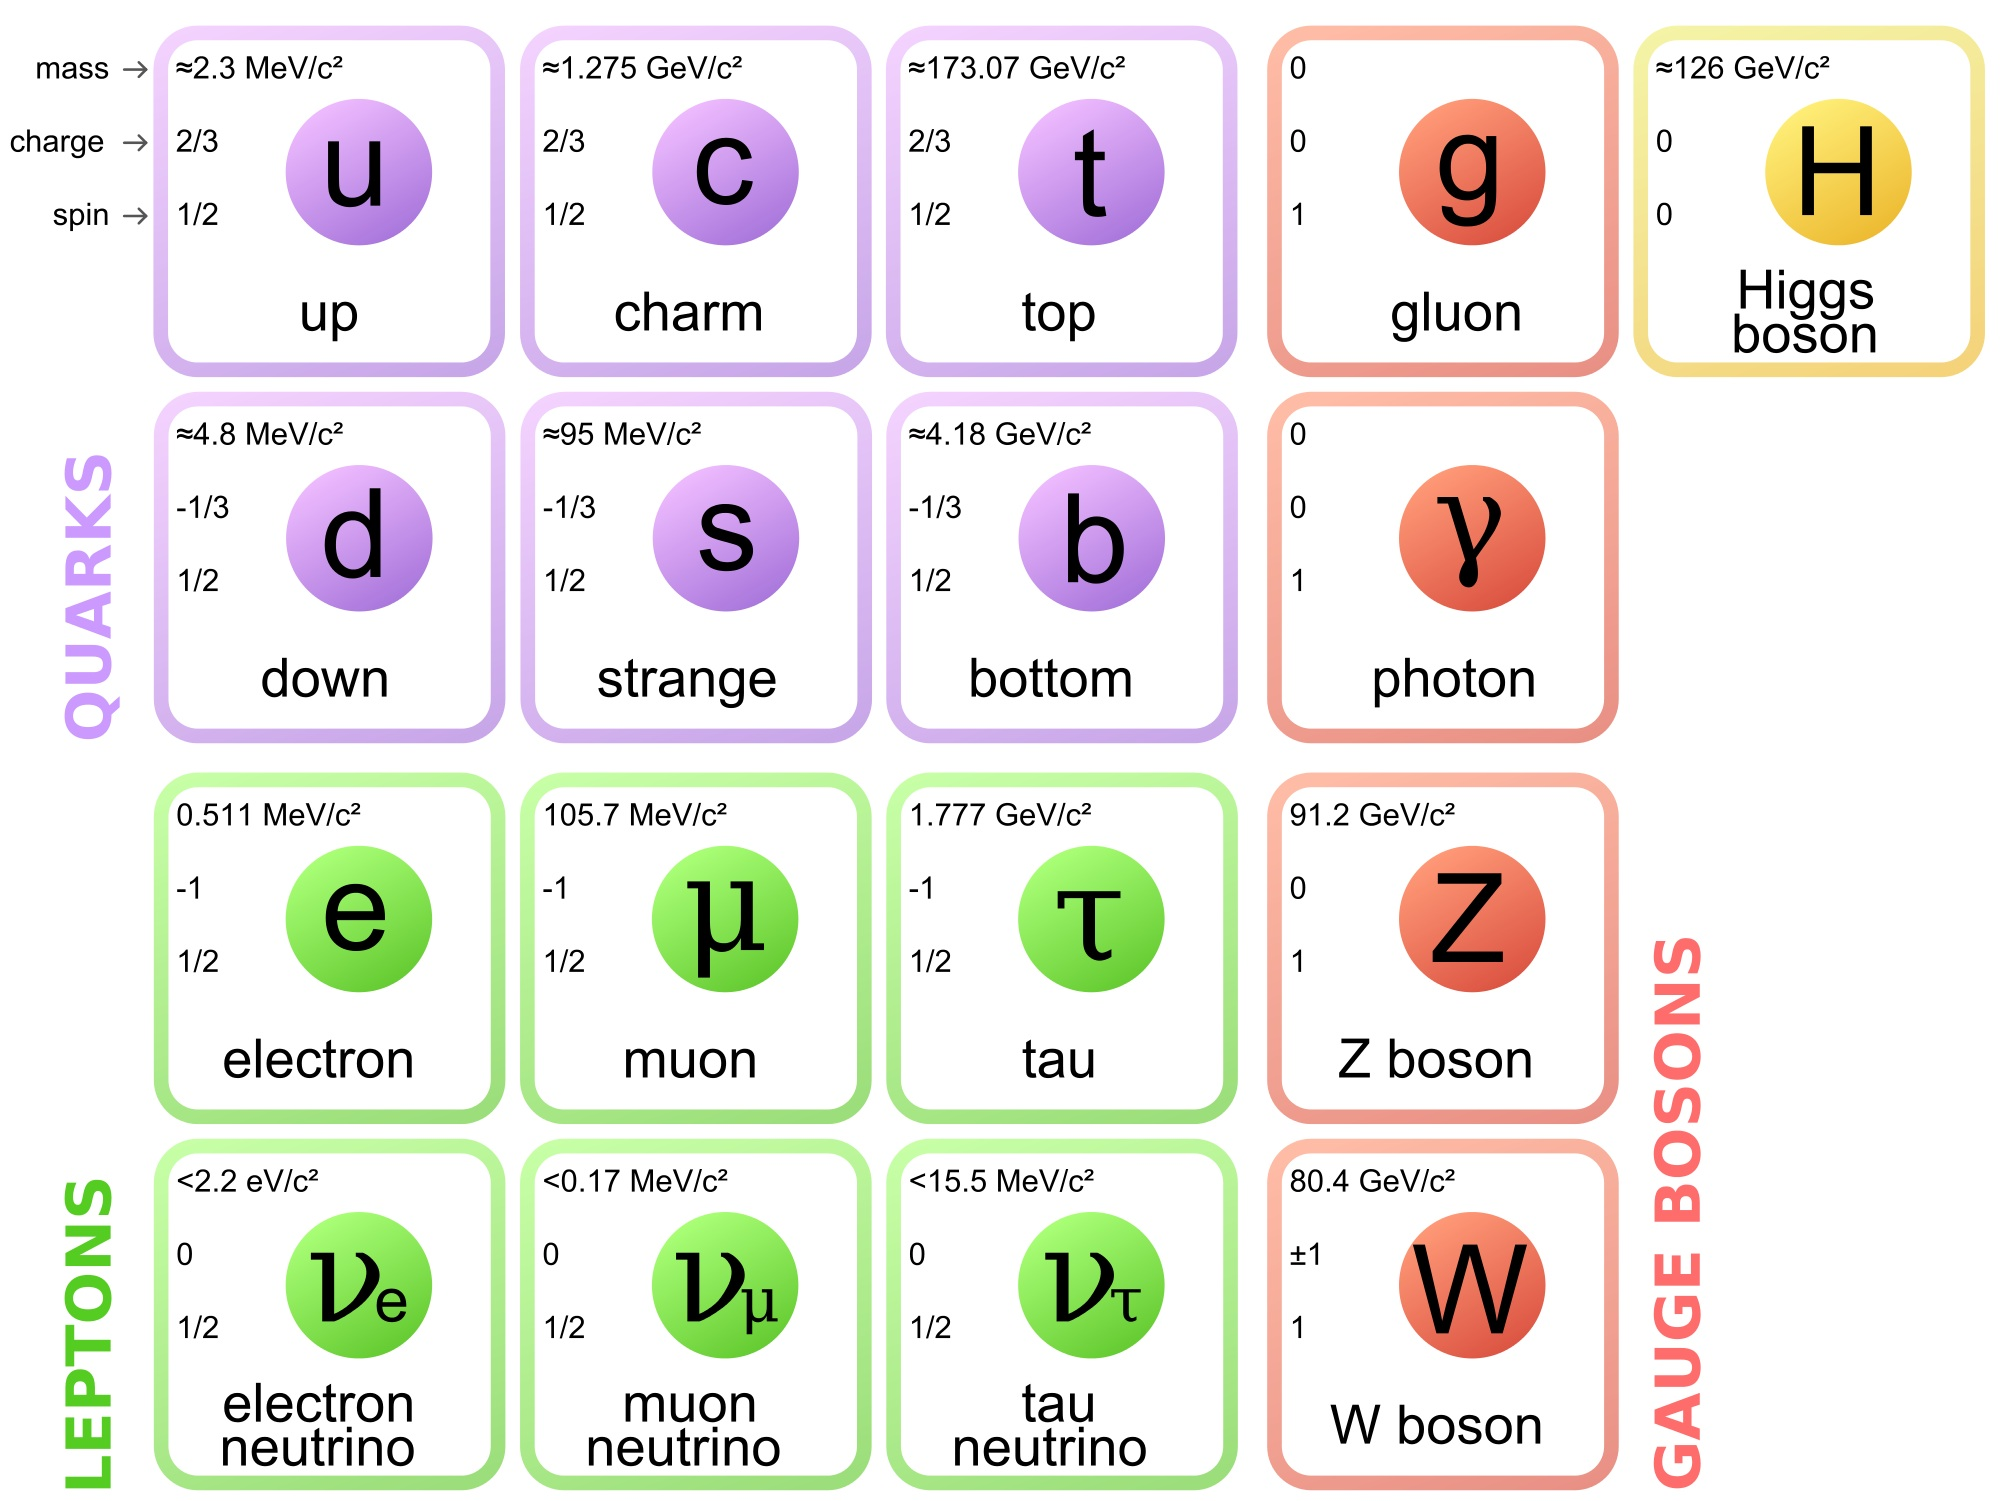
\includegraphics[width=0.75\textwidth]{figs/motivation/SM.jpg}
    \caption{The Standard Model of Particle Physics is a group of the known elementary particles which is composed of six quarks, six leptons, four gauge bosons (which are responsible for the three fundamental forces), and the Higgs Boson (which is the origin of mass of many of the fundamental particles).}
    \label{fig:sm}
\end{figure}


%Missing matter has always driven the field of astronomy alongside the understanding of gravity...

%There is compelling evidence for the existence an invisible type of matter in the universe called dark matter. The first reported evidence of a dynamical model involving missing matter in the universe dates back to Lord Kelvin in the 1800s... Henri Poincare' proposed ``matiere obscure''.

%One could suppose that, since no independent tests of gravity are applied at the galactic scale, that gravity could be wrong. This is a possibility, in fact in the history of astronomy there is often the tension between a new theory of gravity and the presence of some form of unseen matter when presented with some form of anomaly. %The former won in cases such as heliocentricity in favor of geocentricity describing the effect of ``epicycles'' during the times of Copernicus and the orbit of Mercury being explained by Einstein's General Relativity as opposed to Newton's theory of universal gravitation. The latter won in the case with the discovery of Uranus. Though various theories of modified gravity such as Modified Newtonian Dynamics (MoND) or TEVAS successfully resolve the problem of galactic rotation curves, it fails to account for observations from weak gravitation lensing.

%\begin{figure}
%    \centering
%    
\includegraphics[width=0.5\textwidth]{figs/placeholder.jpg}
%    \caption{This is my current placeholder figure.}
%    \label{fig:dm}
%\end{figure}